\documentclass[10pt,a4paper]{article}
\usepackage[margin=20mm]{geometry}
\usepackage{graphicx,array,amsmath,xcolor,hyperref}
\graphicspath{{./}{report/}}
\definecolor{ink}{HTML}{173BDF}
\hypersetup{colorlinks=true,linkcolor=ink,urlcolor=ink,pdftitle={Physics-Guided Search Space Design for Short-Term Photovoltaic Power Forecasting},pdfauthor={Felix Lan}}
\newcommand{\toprule}{\noalign{\hrule height .7pt\vskip3pt}}
\newcommand{\midrule}{\noalign{\vskip2pt\hrule height .4pt\vskip2pt}}
\newcommand{\bottomrule}{\noalign{\vskip3pt\hrule height .7pt}}
\newcommand{\captionof}[2]{\refstepcounter{#1}\par\smallskip{\small\textbf{\csname #1name\endcsname~\csname the#1\endcsname.} #2\par}}
\setlength{\parindent}{0pt}
\setlength{\parskip}{5pt}
\renewcommand{\arraystretch}{1.16}
\setlength{\tabcolsep}{5pt}
\newcommand{\xfig}[1]{figures/20261004_174129_971008_physics_tpe/#1.pdf}
\newcommand{\cfig}[1]{figures/20261025_CNN_LSTM/#1.pdf}
\begin{document}
{\LARGE\bfseries\raggedright Physics-Guided Search Space Design for Short-Term Photovoltaic Power Forecasting\par}

\section{Research question}
Photovoltaic (PV) power depends on irradiance, temperature and conversion efficiency, yet these quantities are partly redundant and related nonlinearly. Adding every measured and derived variable enlarges the feature search without guaranteeing more useful information. A physical model can instead guide which combinations are worth searching: AC and DC power share much of their information, whereas cell temperature and time of day describe different aspects of PV operation.

Building on physics-informed feature selection for PV forecasting\footnote{Pombo et al., \textit{Energy Reports} 8 (2022), 6512--6520. \href{https://doi.org/10.1016/j.egyr.2022.05.006}{doi:10.1016/j.egyr.2022.05.006}.}, this study examines whether a physically relevant, nonredundant candidate space yields better forecasts after joint configuration search. Physics determines the allowable inputs; optimization then selects the subset, history length and model settings. The comparison therefore concerns how the search space is designed, rather than the isolated effect of adding one physical variable.

\section{Data and preprocessing}
The \href{https://doi.org/10.11583/DTU.17040767}{SOLETE dataset} provides inverter AC power and meteorological measurements at five-minute intervals from the SYSLAB installation at DTU Risø, Denmark. The available file spans 1 June 2018 to 1 September 2019 (131,617 timestamps); solar geometry uses UTC at $55.6867^\circ$ N, $12.0985^\circ$ E. Raw measured power can differ from available PV power, for example during curtailed operation. The forecasting target is the physically corrected available-power series; raw measurements are retained for sensitivity analysis. The corrected series also supplies the historical power input.

Timestamps were sorted onto a regular grid, duplicate timestamps rejected, and forecast windows spanning missing or invalid inputs excluded. Plane-of-array irradiance $G$ (W/m$^2$), ambient temperature and wind speed $v$ were used to estimate module and cell temperatures:
\[
T_{\rm module}=T_{\rm ambient}+G\exp(-3.56-0.075v),\qquad
T_{\rm cell}=T_{\rm module}+3G/1000.
\]
DC power was calculated from irradiance and cell temperature for a 7.2 kW array (36 modules of 200 W), with a temperature coefficient of $-0.00478\,{}^{\circ}\mathrm{C}^{-1}$ relative to $25\,{}^{\circ}\mathrm{C}$. A conversion efficiency of 0.98 and a 10 kW AC cap gave the Pac estimate. MinutesOfDay and HoursOfDay were derived from timestamps.

Measured power was replaced by Pac when Pac exceeded 0.05 kW and the absolute discrepancy exceeded 20\% of Pac. Missing power was replaced where Pac was finite, and corrected values at or below 0.001 kW were set to zero. The original TRAIN/VAL/TEST timestamp partitions contained 3,453/1,440/760 changed rows, respectively.

Data were divided chronologically into 70\% TRAIN, 20\% VAL and 10\% TEST, yielding 91,951, 26,265 and 13,103 eligible forecast origins under the common-history requirement. Scaling and correlation selection used TRAIN only. Night observations remained in continuous histories; primary VAL and TEST scores retained only geometric daylight at each target timestamp.

\section{Feature search-space design}
The four spaces differ in their allowable inputs (Table~\ref{tab:spaces}). Original uses measured meteorology; Expanded-Pearson screens expanded candidates by TRAIN correlation. Expanded-Physics avoids redundant pairs such as Pac/Pdc and module/cell temperature while retaining physically complementary inputs. Intrinsic uses power history alone.

\begin{table}[htbp]
\centering\small
\begin{tabular}{@{}lp{11.5cm}@{}}\toprule
Space & Optional inputs in addition to corrected power history \\\midrule
Original & Air temperature, humidity, wind speed/direction, GHI and POA irradiance \\
Expanded-Pearson & Expanded candidates with absolute TRAIN Pearson correlation with the target $\geq 0.70$; humidity retained by override \\
Expanded-Physics & Humidity, POA irradiance, Pac, TempCell and HoursOfDay \\
Intrinsic & None \\\bottomrule
\end{tabular}
\caption{Candidate inputs in each search space. All spaces include corrected power history.}\label{tab:spaces}
\end{table}

Pearson screening retained seven optional candidates: GHI, POA, Pac, Pdc, TempModule, TempCell and humidity. Humidity ($|r|=0.5903$) was retained by a predeclared override to preserve an atmospheric-moisture descriptor alongside the irradiance and conversion features; it did not meet the correlation threshold. Each trial then selected a subset within its declared space.

\section{Models and experimental procedure}
XGBoost fitted one regressor per forecast step. CNN-LSTM combined causal convolution, pooling and LSTM layers with a linear 60-output head. Persistence repeated current power. All models predicted 5 minutes to 5 hours ahead on common TEST origins.

\begin{figure}[htbp]
\centering
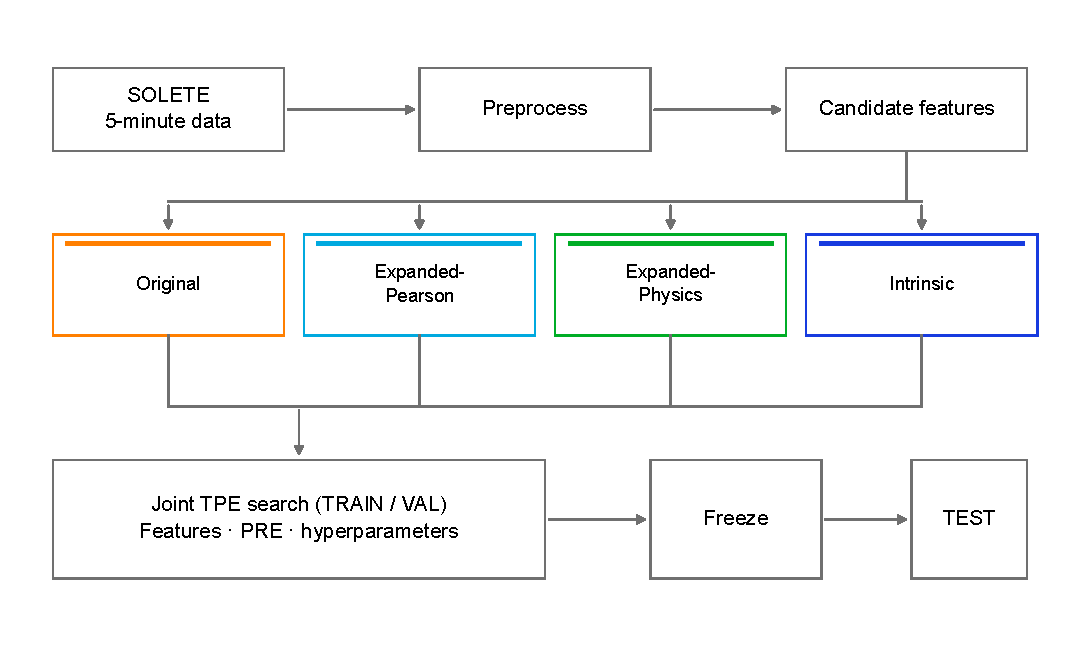
\includegraphics[width=.53\linewidth]{figures/experimental_framework.pdf}
\caption{Experimental workflow. Each space is optimized independently; selected configurations are frozen before TEST evaluation.}\label{fig:workflow}
\end{figure}

Optuna TPE jointly searched feature subsets, PRE and model hyperparameters, with seed 11. PRE counts past samples plus a separate current observation, up to 120 past samples (10 hours). XGBoost received 40 attempts per space, including failures, with ten startup attempts; tree depth, learning rate, regularization and sampling were varied. CNN-LSTM received two attempts per space on 4,096 TRAIN and 1,024 VAL windows, with a 40-epoch cap and patience of eight. Its search considered PRE=30 or 60, convolutional size, LSTM width and learning rate.

CNN-LSTM checkpoints minimized all-hour scaled VAL MAE. Final configurations minimized mean-horizon daylight VAL RMSE in kW. Winners were frozen before one TEST evaluation; no TEST-driven retuning was performed.

For daylight targets $D_h$ at horizon $h$, the primary score was
\[
\mathrm{RMSE}_h=\sqrt{\frac{1}{|D_h|}\sum_{i\in D_h}(\hat y_{i,h}-y_{i,h})^2},\qquad
\overline{\mathrm{RMSE}}=\frac{1}{60}\sum_{h=1}^{60}\mathrm{RMSE}_h.
\]
MAE and $R^2$ were also horizon-averaged; nRMSE was $100\,\overline{\mathrm{RMSE}}/(10\,\mathrm{kW})$.

\clearpage
\section{Search and training results}
\subsection*{XGBoost}
Expanded-Physics achieved the lowest selected VAL RMSE, 0.9732 kW, using TempCell and HoursOfDay with PRE=110 (Table~\ref{tab:xgb}). Pac was not selected, so the observed gain cannot be attributed simply to including theoretical power. The Pearson-space winner used GHI and TempCell. Intrinsic had the highest selected VAL RMSE among the four spaces.

\begin{figure}[htbp]
\centering
\includegraphics[width=.70\linewidth]{\xfig{optimization_progress}}
\caption{XGBoost best-so-far daylight VAL RMSE. Original attempts 15--24 carry forward the previous best value; no successful scores were imputed.}\label{fig:search}
\end{figure}

\begin{table}[htbp]
\centering\small
\begin{tabular}{@{}llrrr@{}}\toprule
Space & Selected optional inputs & PRE & VAL RMSE (kW) & Fits \\\midrule
Original & GHI & 120 & 0.9911 & 30/40 \\
Expanded-Pearson & GHI, TempCell & 120 & 0.9903 & 40/40 \\
Expanded-Physics & TempCell, HoursOfDay & 110 & 0.9732 & 40/40 \\
Intrinsic & None & 110 & 1.0104 & 40/40 \\
\bottomrule\end{tabular}
\caption{Selected XGBoost configurations. VAL RMSE uses daylight targets from all 26,265 eligible VAL windows. Fits denotes successful fits out of 40 attempts.}\label{tab:xgb}
\end{table}

In Original, Expanded-Pearson, Expanded-Physics and Intrinsic order, the selected maximum tree depths were 5, 5, 5 and 6, and learning rates were 0.02854, 0.01362, 0.01753 and 0.02222, respectively.

Original completed 30 fits, compared with 40 in every other space. Nine attempts failed a source/Git compatibility check and one was interrupted. They remained in the declared budget, giving equal attempt counts but unequal numbers of successful fits.

\clearpage
\subsection*{CNN-LSTM}
Expanded-Physics also obtained the lowest selected VAL RMSE for CNN-LSTM, 1.3677 kW (Table~\ref{tab:cnn}). All selected networks used 16 convolutional filters, one 10-unit LSTM layer and PRE=30, retaining all optional inputs in their respective spaces. The two sampled learning rates were close, approximately 0.000700 and 0.000703; this run therefore explored only a narrow range of configurations.

\begin{figure}[htbp]
\centering
\includegraphics[width=.70\linewidth]{\cfig{training_curves}}
\caption{CNN-LSTM VAL MAE on scaled targets at each epoch. Curves end at the actual stopping epoch and use the recorded values without smoothing.}\label{fig:training}
\end{figure}

\begin{table}[htbp]
\centering\small
\begin{tabular}{@{}lrrrr@{}}\toprule
Space & PRE & Best epoch & Stop epoch & VAL RMSE (kW) \\\midrule
Original & 30 & 20 & 28 & 1.5616 \\
Expanded-Pearson & 30 & 12 & 20 & 1.5219 \\
Expanded-Physics & 30 & 40 & 40 & 1.3677 \\
Intrinsic & 30 & 12 & 20 & 1.6317 \\
\bottomrule\end{tabular}
\caption{Selected CNN-LSTM checkpoints and stopping epochs. VAL RMSE uses daylight targets from 1,024 sampled VAL windows, rather than the full VAL partition used for XGBoost. Checkpoint selection uses scaled MAE.}\label{tab:cnn}
\end{table}

All selected CNN-LSTM configurations used a convolutional kernel size of 3, pooling size of 2, batch size of 64 and the Adam optimizer with gradient clipping at norm 1. Learning rates were 0.000700 for Original and Expanded-Pearson, and approximately 0.00070334 for Expanded-Physics and Intrinsic.

Original, Pearson and Intrinsic reached validation plateaus or later increases and stopped after their best checkpoints. Physics continued improving through epoch 40, so convergence was not established. These epoch-loss curves describe training, whereas the XGBoost trace describes configuration search; their values and rates of decrease are not directly comparable.

\clearpage
\section{Test-set forecasting performance}
Expanded-Physics gave the lowest mean TEST RMSE within both model families (Table~\ref{tab:test}). Relative to Original, RMSE decreased from 1.0151 to 0.9536 kW for XGBoost (6.06\%) and from 1.4615 to 1.2383 kW for CNN-LSTM (15.27\%). Expanded-Pearson did not improve on Original for XGBoost, and Intrinsic outperformed both Original and Expanded-Pearson, indicating that increasing the candidate set alone was insufficient.

\begin{table}[htbp]
\centering\small
\begin{tabular}{@{}llrrrr@{}}\toprule
Model & Space & MAE (kW) & RMSE (kW) & nRMSE (\%) & $R^2$ \\\midrule
Persistence & Baseline & 1.2516 & 1.6791 & 16.79 & -0.1171 \\
\midrule
XGBoost & Original & 0.6578 & 1.0151 & 10.15 & 0.6183 \\
XGBoost & Expanded-Pearson & 0.6673 & 1.0184 & 10.18 & 0.6156 \\
XGBoost & Expanded-Physics & 0.6175 & 0.9536 & 9.54 & 0.6644 \\
XGBoost & Intrinsic & 0.6570 & 0.9888 & 9.89 & 0.6385 \\
\midrule
CNN-LSTM & Original & 1.0542 & 1.4615 & 14.61 & 0.1991 \\
CNN-LSTM & Expanded-Pearson & 1.0358 & 1.4433 & 14.43 & 0.2034 \\
CNN-LSTM & Expanded-Physics & 0.8565 & 1.2383 & 12.38 & 0.4242 \\
CNN-LSTM & Intrinsic & 1.0847 & 1.5249 & 15.25 & 0.0836 \\
\bottomrule\end{tabular}
\caption{Daylight TEST metrics against the corrected target, averaged over 60 horizons. Persistence is shared across the two runs.}\label{tab:test}
\end{table}

\begin{figure}[htbp]
\centering
\includegraphics[width=.49\linewidth]{\xfig{forecast_horizon_error}}\hfill
\includegraphics[width=.49\linewidth]{\cfig{forecast_horizon_error}}
\caption{RMSE at each forecast horizon for XGBoost (left) and CNN-LSTM (right). Black denotes Persistence; colored curves identify feature spaces.}\label{fig:horizons}
\end{figure}

The benefit of physics-guided search depended on the comparator and forecast horizon (Fig.~\ref{fig:horizons}). Expanded-Physics achieved lower TEST RMSE than Original at all 60 horizons for both models. Within CNN-LSTM, it outperformed Intrinsic at 53 of 60 horizons and Persistence at 58 of 60. For CNN-LSTM at five minutes, Physics RMSE was 0.6313 kW, above Persistence at 0.5588 kW. This short-lead result is consistent with recent power observations remaining highly informative, leaving less room for additional features to improve forecasts.

The first TEST days illustrate behavior at individual timestamps (Fig.~\ref{fig:examples}). The XGBoost example uses a five-minute lead and CNN-LSTM a one-hour lead; their visual agreement cannot establish a model ranking. CNN-LSTM forecasts included peak errors, lag and negative outputs. CNN-LSTM Physics produced negative values at 12.9\% of evaluated daylight targets before constraints; these outputs were retained in the primary scores.

\begin{figure}[htbp]
\centering
\includegraphics[width=.59\linewidth]{\xfig{prediction_curves}}\par
\includegraphics[width=.59\linewidth]{\cfig{prediction_curves}}
\caption{First 864 retained target timestamps: XGBoost at five minutes (top) and CNN-LSTM at one hour (bottom). Black curves are corrected observations.}\label{fig:examples}
\end{figure}

\begin{figure}[htbp]
\centering
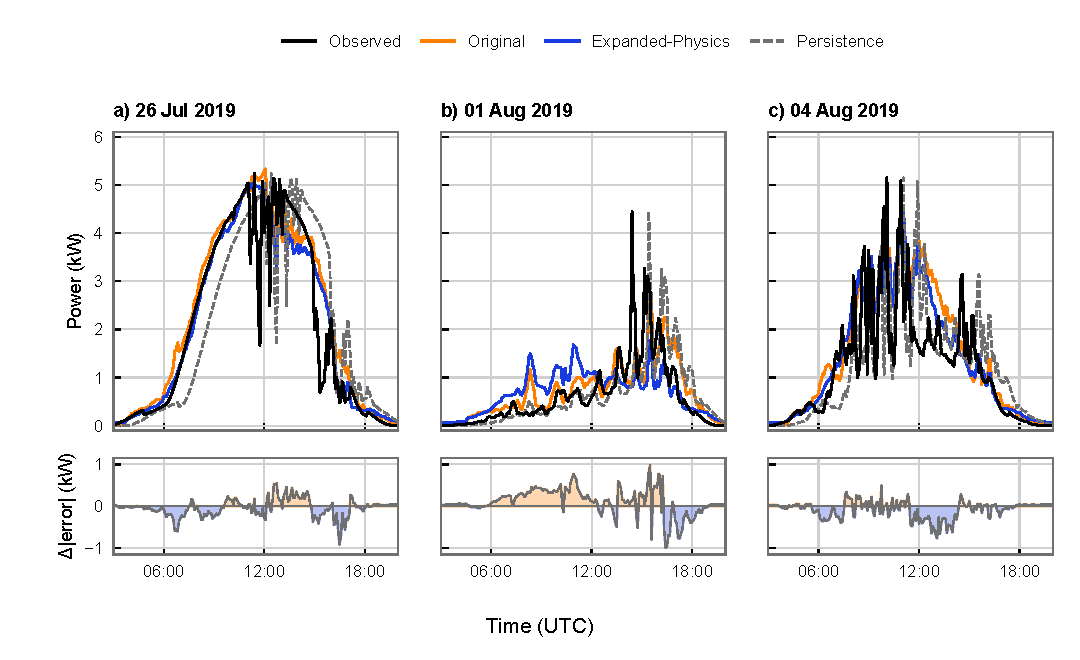
\includegraphics[width=.79\linewidth]{figures/forecast_example.pdf}
\caption{One-hour XGBoost forecasts on dates chosen by measured-power variability, independently of forecast errors. Orange: Original; dark blue: Physics; black: raw measurements; dashed gray: Persistence. Lower strips show $|e_{\rm Physics}|-|e_{\rm Original}|$; negative values favor Physics. In this panel only, Physics is dark blue; it is green in Figs.~\ref{fig:workflow}--\ref{fig:examples}, where dark blue denotes Intrinsic.}\label{fig:hour}
\end{figure}

\clearpage
\section{Robustness, limitations and conclusions}
Physics remained better than Original when the frozen forecasts were scored against raw measured power (Table~\ref{tab:raw}). For XGBoost, raw-target RMSE was 0.9551 versus 1.0172 kW; for CNN-LSTM, it was 1.2341 versus 1.4632 kW. The advantage thus persisted under a change of scoring target, although training and configuration selection still depended on the correction rules.

\begin{table}[htbp]
\centering\small
\begin{tabular}{@{}llrr@{}}\toprule
Model & Space & Raw-target MAE (kW) & Raw-target RMSE (kW) \\\midrule
XGBoost & Original & 0.6600 & 1.0172 \\
XGBoost & Expanded-Pearson & 0.6705 & 1.0215 \\
XGBoost & Expanded-Physics & 0.6186 & 0.9551 \\
XGBoost & Intrinsic & 0.6562 & 0.9885 \\
\midrule
CNN-LSTM & Original & 1.0525 & 1.4632 \\
CNN-LSTM & Expanded-Pearson & 1.0330 & 1.4436 \\
CNN-LSTM & Expanded-Physics & 0.8493 & 1.2341 \\
CNN-LSTM & Intrinsic & 1.0798 & 1.5231 \\
\bottomrule\end{tabular}
\caption{Sensitivity to raw measured targets, using the same frozen forecasts and daylight evaluation masks.}\label{tab:raw}
\end{table}

Paired circular block bootstrap intervals for Physics-minus-baseline MAE differences were below zero for all six aggregate comparisons in Table~\ref{tab:ci}. This does not hold for every horizon-specific interval. Errors were first averaged by forecast origin, then resampled in blocks of 288 origins with 2,000 replicates. This weighting differs from the horizon averages in Table~\ref{tab:test}, so the differences need not equal direct subtraction of its entries. Intervals represent temporal uncertainty in the retained predictions, not variability across retraining seeds; no multiplicity correction was applied.

\begin{table}[htbp]
\centering\small
\begin{tabular}{@{}llrr@{}}\toprule
Model & Baseline & $\Delta$MAE (kW) & 95\% interval (kW) \\\midrule
XGBoost & Original & -0.0375 & [-0.0555, -0.0188] \\
XGBoost & Expanded-Pearson & -0.0442 & [-0.0589, -0.0295] \\
XGBoost & Intrinsic & -0.0347 & [-0.0555, -0.0129] \\
\midrule
CNN-LSTM & Original & -0.1818 & [-0.2137, -0.1514] \\
CNN-LSTM & Expanded-Pearson & -0.1653 & [-0.1940, -0.1371] \\
CNN-LSTM & Intrinsic & -0.1959 & [-0.2212, -0.1688] \\
\bottomrule\end{tabular}
\caption{Physics minus baseline MAE and 95\% block-bootstrap intervals, based on 11,056 origins with evaluated targets. Negative differences favor Physics.}\label{tab:ci}
\end{table}

Two mechanisms may contribute to the observed gains. Physical features can encode the nonlinear relationships among irradiance, temperature and power in a form that is easier to learn. Excluding redundant candidates may also concentrate a fixed search budget on useful configurations. Neither mechanism was isolated experimentally, and their contributions may depend on the forecasting conditions. The measured benefit therefore belongs to the joint search procedure, rather than to any single physical feature; improved search efficiency has not been established.

The advantage was consistent within the recorded experiments, including raw-target scoring, but robustness across independent repetitions remains untested. Only one seed, site and TEST period were assessed. CNN-LSTM used a small-sample diagnostic budget, preventing a direct model-family ranking, and its Physics configuration was still improving at the epoch cap. Failed XGBoost Original attempts reduced its effective search exposure. CNN-LSTM development followed inspection of XGBoost TEST results, so it was not prospectively blinded.

\end{document}
